%
% main.tex -- Paper zum Thema <julia>
%
% (c) 2020 Autor, OST Ostschweizer Fachhochschule
%
% !TEX root = ../../buch.tex
% !TEX encoding = UTF-8
%
\chapter{Julia-Mengen und Mandelbrot-Menge\label{chapter:julia}}
\kopflinks{Julia-Mengen und Mandelbrot-Menge}
\begin{refsection}
\chapterauthor{Nicola Dall'Acqua}

\noindent
Julia-Mengen und die Mandelbrot-Menge entstehen, wenn Kompositionen von holomorphen Funktionen mit sich selbst betrachtet werden.
Konkret wird untersucht, wie sich Funktionen verhalten, wenn diese wiederholt auf sich selbst angewendet werden.
Dieses Gebiet wird auch als \emph{komplexe Dynamik} oder \emph{holomorphe Dynamik} bezeichnet.
\index{komplexe Dynamik}%
\index{holomorphe Dynamik}%
\index{Dynamik, komplex}%
\index{Dynamik, holomorph}%

Das Interesse an dieser Idee lässt sich beispielsweise mit numerischen Methoden, wie dem Newton-Algorithmus motivieren.
\index{Newton-Algorithmus}%
Dieser kann zur Lösung der Gleichung
\begin{equation}
    x^2 + a = 0
    \label{julia:beispielgleichung}
\end{equation}
herangezogen werden.
Die Iterationsformel lautet
\begin{equation}
    x_{n + 1} = x_n - \frac{f(x_n)}{f^\prime(x_n)} = x_n - \frac{x_n^2 + a}{2x_n} = g(x_n).
    \label{julia:newton_alg}
\end{equation}
Was sich hinter dieser Formel verbirgt, ist nichts weiter als eine Komposition von einer Funktion $g$ mit sich selbst --- man erhält den nächsten Wert $x_{n + 1}$, indem man die Funktion $g$ auf den aktuellen Wert $x_n$ anwendet.

Wird nun der Startwert $x_0$ genügend nahe an der exakten Lösung von der Gleichung \eqref{julia:beispielgleichung} gewählt, wird die Iterationsfolge $x_n$ gegen die Lösung konvergieren.
Anders sieht es aus, wenn der Startwert weit weg von der exakten Lösung gewählt wird.
Zudem besitzt diese Gleichung einen Parameter $a$.
Ist $a = 1$, so erreicht der Newton-Algorithmus in den reellen Zahlen gar keine Konvergenz.
Die Iteration der Funktion $g$ kann sich also, basierend auf verschiedenen Umständen, auf verschiedene Weisen verhalten.

Für das genaue Verständnis der Folge $x_0,\, x_1,\, x_2,\, \ldots,$ welche durch die Iteration von $g$ entsteht, müssen also Hilfsmittel entwickelt werden.
Dies führt schlussendlich zu den Julia-Mengen und den Fatou-Mengen, welche das Komplement der Julia-Mengen sind, sowie der Mandelbrot-Menge.

In den Abschnitten \eqref{julia:sec:julia} und \eqref{julia:sec:mandelbrot} werden zunächst Julia- und Fatou-Mengen sowie die Mandelbrot-Menge definiert.
Anschliessend wird im Abschnitt \eqref{julia:zweck} die Frage nach dem Verhalten der Newton-Iterationsfolge \eqref{julia:newton_alg} beantwortet.
Weiter werden verschiedene Zusammenhänge zwischen all diesen Mengen im Abschnitt \eqref{julia:sec:relation} untersucht.
Abschliessend wird im Abschnitt \eqref{julia:sec:visualisierung} beschrieben, wie man diese Mengen darstellen kann.

\section{Julia-Mengen und Fatou-Mengen}
\label{julia:sec:julia}
\kopfrechts{Julia-Mengen und Fatou-Mengen}%
Julia-Mengen und Fatou-Mengen entstehen aus der Überlegung was geschieht, wenn man eine komplexe Funktion $f$ wiederholt auf ein $z \in \mathbb{C}$ anwendet.
Hieraus ergibt sich für jedes $z$ eine Folge komplexer Zahlen
\begin{equation}
    z \rightarrow f(z) \rightarrow f(f(z)) \rightarrow \ldots \:,
    \label{julia:julia_folge}
\end{equation}
bzw.
\begin{equation*}
    z_{n + 1} = f(z_n) \quad \text{mit}\: n \in \mathbb{N}_0\: \text{und einem Startwert}\: z_0 \in \overline{\mathbb{C}} = \mathbb{C} \cup \infty.
\end{equation*}

Je nach Wahl des Startwerts $z_0$ kann diese Folge zwei Verhalten zeigen:
\begin{enumerate}
    \item Eine kleine Änderung des Startwerts führt zur praktisch derselben Folge. Der Wert $z_0$ wird der \emph{Fatou-Menge} $F_f$ von $f$ zugeordnet.
\index{Fatou-Menge}%
    \item Eine kleine Änderung des Startwerts führt zu einer komplett anderen Folge. In diesem Fall wird $z_0$ der \emph{Julia-Menge} $J_f$ von $f$ zugeordnet.
\index{Julia-Menge}%
\end{enumerate}
Innerhalb dieses Abschnitts sollen die obigen, provisorischen Definitionen formalisiert werden.

Die Begriffe ``praktisch dieselbe Folge'' und ``komplett andere Folge'' beziehen sich darauf, gegen welche Werte die Folgen gehen, wenn $n \to \infty$.
Weiter ist mit ``eine kleine Änderung'' gemeint, dass ein $\varepsilon \in \mathbb{C}$ mit $|\varepsilon|$ nahe bei $0$ zum Startwert $z_0$ addiert wird.
Wenn es für einen Startwert ein $\varepsilon$ gibt, so dass man eine komplett andere Folge erhält, so gehört der Startwert zur Julia-Menge, auch wenn es andere $\varepsilon$ gibt, für die dies nicht der Fall ist.

\subsection{Periodische Folgen}
Das Verhalten von solchen Folgen ist besonders dann interessant, wenn diese periodisch sind, bzw. $z_n = z_0$ für ein $n > 0$ gilt.
In dem Fall wird $z_0$ als \emph{periodischer Punkt} bezeichnet.
\index{periodischer Punkt}%
Ist $n$ die kleinste natürliche Zahl mit dieser Eigenschaft, so heisst $n$ die \emph{Periode} des Zyklus.
\index{Periode}%
Falls dies bereits für $n = 1$ zutrifft, wenn also $f(z_0) = z_0$ gilt, so ist $z_0$, nicht nur ein periodischer Punkt, sondern auch ein \emph{Fixpunkt} von $f$.
\index{Fixpunkt}%
Aus diesen Definitionen geht hervor, dass ein periodischer Punkt von $f$ mit Periode $n$ gleichzeitig ein Fixpunkt der $n$-fach zusammengesetzten Funktion $f^n$ ist.

Um die Komplexität der Fragestellung zu reduzieren, werden zunächst nur Fixpunkte betrachtet.

\subsubsection{Anziehende und abstossende Fixpunkte}
Am Beispiel der Funktion 
\begin{equation*}
    f(z) = z^2,
\end{equation*}
lassen sich zwei verschiedene Verhaltensweisen von Fixpunkten beobachten.

Durch $n$-maliges Anwenden erhält man $f^n(z) = z^{2^n}$.
Weiter hat die Funktion $f$ drei Fixpunkte: $0, 1$ und $\infty$, denn für diese Punkte gilt $f(z_0) = z_0$.

Entwickelt man nun die Folge \eqref{julia:julia_folge} ausgehend von den Startwerten $0$ und $\infty$, so erhält man $f^n(0) = 0$ bzw. $f^n(\infty) \to \infty$.
Nun werden diese Startwerte leicht verändert, dies geschieht mittels einem $\varepsilon \in \mathbb{C}$, wobei $|\varepsilon|$ nahe bei $0$ ist:
\begin{itemize}
    \item Für $z_0 = 0$: $f^n(0 + \varepsilon) = (0 + \varepsilon)^{2^n} \to 0$ mit $|\varepsilon| > 0$
    \item Für $z_0 \to \infty$: $f^n(\infty + \varepsilon) = (\infty + \varepsilon)^{2^n} \to \infty$ mit $|\varepsilon| > 0$
\end{itemize}
Obwohl die Startwerte verändert wurden, erhält man schlussendlich die gleichen Resultate, wie wenn man die Startwerte nicht verändert hätte.
Anders ausgedrückt führen kleine Änderungen der Startwerte zu praktisch denselben Folgen.
Es scheint, dass diese beiden Startwerte Folgen in ihrer Umgebung anziehen, sprich dass es sich um \emph{anziehende} Fixpunkte handelt.
\index{anziehend}%
\index{Fixpunkt!anziehend}%

Für den Startwert $1$ erhält man $f^n(1) = 1$, durch leichtes Verändern jedoch:
\begin{itemize}
    \item $f^n(1 + \varepsilon) = (1 + \varepsilon)^{2^n} \to \infty$
    \item $f^n(1 - \varepsilon) = (1 - \varepsilon)^{2^n} \to 0$
\end{itemize}
Hier scheint es also, dass eine kleine Änderung des Startwerts zu einer ganz anderen Folge führt, heisst es handelt sich um einen \emph{abstossenden} Fixpunkt.
\index{Fixpunkt!abstossend}%

\subsubsection{Indifferente Fixpunkte}
Als zweites Beispiel dient die Funktion
\begin{equation*}
    h(z) = z + z^7,
\end{equation*}
bei der sich indifferente Fixpunkte beobachten lassen.
Diese Funktion hat Fixpunkte bei $-\infty, 0$ und $\infty$.
Die Fixpunkte $-\infty$ und $\infty$ verhalten sich erneut anziehend und werden daher nicht näher untersucht.
Nimmt man jedoch $0$ als Startwert, passiert etwas anderes.
Zunächst ergibt sich $h^n(0) = 0$, durch eine kleine Änderung erhält man,
\begin{equation*}
    h(0 + \varepsilon) = (0 + \varepsilon) + (0 + \varepsilon)^7.
\end{equation*}
Da es sich bei $|\varepsilon|$ um eine sehr kleine Zahl handelt, ist der zweite Summand gegenüber $\varepsilon$ vernachlässigbar, übrig bleibt der lineare Term.
Somit ist
\begin{equation*}
    h(0 + \varepsilon) \approx 0 + \varepsilon.
\end{equation*}
Wendet man nun erneut $h$ auf dieses Resultat an, erhält man wieder $0 + \varepsilon$.
Auch durch $n$-maliges Anwenden von $h$ ändert sich das Resultat nicht.
Die Folge ``bewegt'' sich also, anders als vorhin, nicht.
Der Startwert $0$, scheint also Folgen weder abzustossen, noch anzuziehen, man bezeichnet den Fixpunkt daher als \emph{indifferent}.
\index{Fixpunkt!indifferent}%

\subsubsection{Arten von Fixpunkten}
\label{julia:arten_periodische_punkte}
Das Verhalten einer Folge hängt also von der Art des verwendeten Fixpunktes ab.
Sei $z_0$ ein periodischer Punkt von $f$ mit Periode $n$, demzufolge ist $z_0$ ein Fixpunkt von $g = f^n$.
Dadurch wird die Frage nach dem Verhalten in der Nähe eines periodischen Punktes reduziert auf die Frage nach dem Verhalten in der Nähe eines Fixpunktes.
Diese Frage lässt sich mithilfe der Taylor-Reihe um $z_0$
\begin{equation*}
    g(z) \approx z_0 + g^\prime(z_0) (z - z_0)
    \label{julia:taylor}
\end{equation*}
beantworten, wobei höhere Potenzen in der Nähe von $z_0$ vernachlässigbar sind.
Verwendet man $z_0$ als Startwert und ändert diesen leicht, bedeutet dies
\begin{equation*}
    z = z_0 + \varepsilon.
\end{equation*}
Setzt man dies in die Taylor-Reihe ein, erhält man
\begin{equation*}
    g(z) = g(z_0 + \varepsilon) \approx z_0 + g^\prime(z_0) \left((z_0 + \varepsilon) - z_0\right) = z_0 + g^\prime(z_0) \varepsilon.
\end{equation*}
Wird $g$ erneut und wiederholt auf dieses Resultat angewendet, so wird das Verhalten der entstehenden Folge einzig von $g^\prime(z_0)$ festgelegt.
Ist $|g^\prime(z_0)| < 1$, so wird der zweite Summand durch wiederholte Anwendungen immer kleiner und die Folge kehrt zu $z_0$ zurück.
Bei $|g^\prime(z_0)| = 0$ geschieht dies bereits nach der ersten Anwendung von $g$.
Im Fall dass $|g^\prime(z_0)| > 1$ ist, wird der zweite Summand immer grösser und die Folge kehrt nicht zu $z_0$ zurück, sondern konvergiert zu einem anderen Wert.

Wenn $|g^\prime(z_0)| = 1$ ist, ergibt sich ein Spezialfall.
Durch wiederholtes Anwenden scheint das Resultat immer $z_0 + \varepsilon$ zu bleiben, das stimmt aber nicht.
Die Formel \eqref{julia:taylor} für die Taylor-Reihe ignoriert die höheren Potenzen, da diese in den drei anderen Fällen nichts am Ausgang ändern.
Wiederholtes Anwenden der Funktion führt dazu, dass die höheren Potenzen irgendwann nicht mehr vernachlässigt werden dürfen, und im Fall $|g^\prime(z_0)| = 1$ werden sie sogar sehr wichtig.
Das Verhalten der Folge wird hier durch diese höheren Potenzen bestimmt.
Die Folge kann sich so verhalten, wie eine Folge ausgehend von einem \emph{anziehenden} oder \emph{abstossenden} Fixpunkt, sie kann sich aber auch gar nicht ``bewegen''.
Dieses Phänomen wird im Abschnitt \ref{julia:sec:indifferent} näher beschrieben.

\begin{definition}
Der \emph{Multiplikator} eines Fixpunkts ist 
\index{Multiplikator}%
\begin{equation*}
    \lambda = g^\prime(z_0) = \left(f^n\right)^\prime(z_0).
    \label{julia:lambda_multiplicator}
\end{equation*}
Weiter sei $z_0$ ein periodischer Punkt,
dann heisst $z_0$ \emph{stark anziehend}, falls $\lambda = 0$,
\index{stark anziehend}%
\emph{anziehend}, falls $0 < |\lambda| < 1$,
\index{anziehend}%
\emph{indifferent}, falls $|\lambda| = 1$,
\index{indifferent}%
und \emph{abstossend}, falls $|\lambda| > 1$.
\index{abstossend}%
\label{julia:lambda_defs}
\end{definition}

Wendet man dies auf das vorherige Beispiel der Funktion $f(z) = z^2$ bzw. $f^n(z) = z^{2^n}$ an, bekommt man
\begin{equation*}
    \lambda = \left(f^n\right)^\prime(z_0) = 2^n z_0^{2^n - 1}.
\end{equation*}
Für die Fixpunkte von $f$ ergibt dies
\begin{itemize}
    \item $\lambda_0 = 0$,
    \item $\lambda_1 = 2^n$.
\end{itemize}
Somit sind diese Punkte stark anziehend, bzw.~abstossed.

Im Fall des Fixpunkts $\infty$ ist zunächst ein Koordinatenwechsel nötig, da sich dieser ausserhalb der komplexen Zahlenebene auf der Riemannschen Zahlenkugel befindet.
Sei
\begin{equation*}
    w = \frac{1}{z},
\end{equation*}
damit ist
\begin{equation*}
    f(w) = w^2 = \frac{1}{z^2}.
\end{equation*}
Für $w \to 0$ verhält sich $f$ gleich, wie für $z \to \infty$.
Berechnet man nun $\lambda$ unter Berücksichtigung der neuen Koordinate bekommt man
\begin{equation*}
    \lambda = \left(f^n\right)^\prime(w_0) = 2 w_0,
\end{equation*}
was für $w \to 0$, den Wert $0$ ergibt.
Insofern ist auch dieser Fixpunkt stark anziehend.

Die Namensgebungen decken sich also mit dem beobachteten Verhalten von Folgen, ausgehend von diesen Startwerten.
Es scheint, als ob eine Definition für die Julia-Mengen auf abstossenden Fixpunkten aufbauen muss. 

\subsection{Beobachtungen}
\label{julia:sec:beobachtungen}
Wie die vorhergehenden Beispiele zeigen, scheinen, gemäss den provisorischen Definition am Anfang des Abschnitts \ref{julia:sec:julia}, abstossende Fixpunkte zur Julia-Menge der jeweiligen Funktion zu gehören.
Ebenfalls scheinen anziehende Fixpunkte zur Fatou-Menge zu gehören.
Dies reicht jedoch noch nicht zur Definition dieser Mengen aus, denn indifferente Punkte, nicht-fixe periodische Punkte und nicht-periodische Punkte wurden noch nicht genauer betrachtet.

\subsubsection{Indifferente Punkte}
\label{julia:sec:indifferent}
Im Abschnitt \ref{julia:arten_periodische_punkte} wurde beschrieben, dass indifferente periodische Punkte einen Spezialfall bilden.
Abhängig von den höheren Potenzen in der Taylor-Reihe können indifferente Punkte entweder zur Julia-Menge oder zur Fatou-Menge ihrer jeweiligen Funktion gehören.
Wenn diese höheren Potenzen bei $n$-maliger Anwendung von $f$ verschwinden, gehört der indifferente Punkt zur Fatou-Menge.
Wachsen diese jedoch langsam, so verhält sich der indifferente Punkt wie ein abstossender Punkt und gehört daher zur Julia-Menge.
Weitere Details sind im Abschnitt 13 in \cite{julia:indifferente_punkte} beschrieben.

\subsubsection{Nicht-fixe periodische Punkte}
\label{julia:sec:nicht_fix_periodisch}
Bisher wurden nur Fixpunkte, also Punkte mit $f(z_0) = z_0$, und deren Verhalten untersucht.
Nicht-fixe periodische Punkte --- also Punkte mit $f^n(z_0) = z_0$, mit $n > 1$ --- verhalten sich grundsätzlich gleich, auch hier gibt es anziehende, abstossende und indifferente Punkte.

\begin{beispiel}
Nachfolgend wird dies am Beispiel der Funktion $f(z) = z^2$ illustriert.
Am Ende des Abschnitts \ref{julia:arten_periodische_punkte} wurde festgestellt, dass $f$ einen abstossenden Fixpunkt bei $1$ hat.
Diese Funktion hat jedoch weitere abstossende, nicht-fixe periodische Punkte --- wenn $n \to \infty$, sogar unendlich viele.

Damit ein Punkt periodisch, aber nicht fix ist, muss
\begin{equation*}
    f^n(z) = z^{2^n} = z,
\end{equation*}
für ein $n > 1$ gelten.
Betrachtet man die beiden rechten Ausdrücke dieser Gleichung und faktorisiert diese, erhält man
\begin{equation*}
    z \left(z^{2^n - 1} - 1\right) = 0.
\end{equation*}
Periodische Punkte von $f$ sind also:
\begin{itemize}
    \item $z = 0$, wie bereits beschrieben ist dieser Punkt stark anziehend und wird daher nicht weiter betrachtet.
    \item $z^{2^n - 1} = 1$.
\end{itemize}

Bei der zweiten Lösung handelt es sich um Einheitswurzeln $z_e$ des Grades $2^n - 1$, d. h. komplexe Zahlen, welche durch Potenzieren irgendwann $1$ ergeben.
Oder anders formuliert, um Wurzeln dieses Polynoms $2^n - 1$-ten Grades.
Für $n \to \infty$ gibt es unendlich viele Einheitswurzeln, was bedeutet, dass $f$ unendlich viele periodische Punkte hat.

Die Einheitswurzeln $z_e$ sind auch abstossend. Um dies zu zeigen berechnet man
\begin{equation*}
    \lambda = \left(f^n\right)^\prime(z_e) = 2^n z_e^{2^n - 1}.
\end{equation*}
Der zweite Faktor ist, aufgrund der Periodizität, gleich $1$, es bleibt
\begin{equation*}
    \lambda = 2^n 1 = 2^n
\end{equation*}
und weil $\lambda > 1$, handelt es sich um abstossende periodische Punkte.

Die Einheitswurzeln $z_e$ liegen stets auf dem Einheitskreis, d.~h. $|z_e| = 1$.
Wäre dies nicht der Fall, würde der Betrag durch das Potenzieren verschwinden, bzw. ansteigen und somit würde $z_e^{2^n - 1} = 1$ nicht mehr gelten.
Addiert man ein $\varepsilon$ mit Betrag nahe bei $0$ zu $z_e$, ist der Betrag entweder kleiner oder grösser als $1$.
Die Folge, die durch wiederholtes Anwenden von $f$ entsteht, wird nun entweder gegen $0$ oder gegen $\infty$ gehen.
Ohne $\varepsilon$ bewirkt $f$, dass das Argument sich um den Einheitskreis dreht und periodisch zu $1$ zurückkehrt.

Gemäss den provisorischen Definitionen am Anfang des Abschnitts \ref{julia:sec:julia} gehören die Einheitswurzeln daher in die Julia-Menge von $f$.
\end{beispiel}

Somit sind nicht nur abstossende Fixpunkte, sondern auch abstossende periodische Punkte relevant zur Definition der Julia-Mengen.

\subsubsection{Nicht-periodische Punkte}
\label{julia:sec:nicht_periodisch}
Punkte die nicht periodisch sind, können entweder zur Julia-Menge oder zur Fatou-Menge gehören.

\begin{beispiel}
Der Punkt $z_0 = e^{2\pi i\sqrt{2}}$ gehört zur Julia-Menge der Funktion $f(z) = z^2 = r e^{2\pi i(2 \varphi)}$, obwohl er nicht periodisch ist.
Durch $n$-maliges Anwenden wird $f$ zu $f^n(z) = z^{2^n} = r^{2^n} e^{2\pi i(2^n \varphi)}$.
Setzt man den Punkt $z_0$ ein, d.h. setzt $\sqrt{2}$ für $\varphi$ ein, müsste
\begin{equation*}
    2^n \sqrt{2} \equiv \sqrt{2} \mod{2\pi}
\end{equation*}
für ein $n$ gelten, damit $z_0$ periodisch ist.
Dies ist aber nur für $n = 0$ der Fall, was bedeutet dass $z_0$ nicht periodisch ist.

Nimmt man $z_0$ als Startwert für eine Folge und verändert diesen leicht, so gibt es drei Fälle
\begin{itemize}
    \item $|z_0 + \varepsilon| = 1$,
    \item $|z_0 + \varepsilon| < 1$,
    \item $|z_0 + \varepsilon| > 1$.
\end{itemize}
Wendet man nun wiederholt $f$ auf den veränderten Startwert an, so wird sich dieser im ersten Fall um den Einheitskreis ``drehen'' und ist möglicherweise sogar periodisch.
Im zweiten Fall wird der Betrag gegen $0$ gehen und im dritten Fall gegen $\infty$.
Je nach Wert von $\varepsilon$ erhält man unterschiedliche Folgen, das Verhalten ist chaotisch und somit gehört $z_0$ zur Julia-Menge von $f$.

Verwendet man für die gleiche Funktion jedoch $0.5$ als Startwert und verändert diesen leicht, so erhält man $f^n(0.5 + \varepsilon) = (0.5 + \varepsilon)^{2^n}$, was gegen $0$ konvergiert.
Die Folge für den unveränderten Startwert konvergiert ebenfalls gegen $0$, was bedeutet, dass dieser Punkt zur Fatou-Menge von $f$ gehört.
\label{julia:nicht_periodisch_julia}
\end{beispiel}

Nicht-periodische Punkte können sich also auch unterschiedlich verhalten und gehören daher entweder zur Julia-Menge oder zur Fatou-Menge.

\subsection{Definition der Julia-Mengen}
Wie im Abschnitt \ref{julia:sec:beobachtungen} gezeigt wurde, scheint es, dass eine Definition für Julia-Mengen
\begin{itemize}
    \item auf abstossenden periodischen Punkten (nicht nur Fixpunkten) aufbauen muss
    \item sowie indifferente periodische Punkte und nicht-periodische Punkte berücksichtigen muss.
\end{itemize}

\begin{beispiel}
Betrachtet man erneut die Funktion $f(z) = z^2$, so ist bereits bekannt, dass alle abstossenden Punkte in der Julia-Menge enthalten sind.
Alle diese Punkte liegen auf dem Einheitskreis und wie im Abschnitt \ref{julia:sec:nicht_fix_periodisch} beschrieben, gibt es unendlich viele davon.

Diese abstossenden Punkte sind jedoch nicht deckungsgleich mit dem Einheitskreis, es gibt ``Lücken'' auf dem Einheitskreis, welche nicht zu dieser Punktemenge gehören (siehe Beispiel \ref{julia:nicht_periodisch_julia}).
Allerdings ist die Distanz von jeder Lücke zu einem abstossenden Punkt beliebig klein.
Obwohl die ``Lückenpunkte'' selber nicht periodisch sind, verhalten sie sich gleich wie abstossende periodische Punkte weil sie so nahe bei diesen liegen.

Entwickelt man die Folge \eqref{julia:julia_folge} ausgehend von einem ``Lückenpunkt'' $z_l$ und entwickelt dann eine zweite Folge ausgehend von $z_l + \varepsilon$, erhält man ebenfalls zwei komplett andere Folgen.
Für den Startwert $z_l$ führt wiederholtes Anwenden von $f$ auch dazu, dass sich das Argument um den Einheitskreis dreht, jedoch nie mehr zu $1$ zurückkehrt.
Für $z_l + \varepsilon$ geht wiederholtes Anwenden gegen $0$, wenn $|\varepsilon|$ negativ ist und gegen $\infty$, wenn $|\varepsilon|$ positiv ist.
Diese ``Lückenpunkte'' gehören somit auch zur Julia-Menge.

Was die indifferenten periodischen Punkte angeht, so hat die Funktion $f$ keine davon.
Allgemein verhalten sich diese jedoch auch abstossend, wenn sie in einer solchen ``Lücke'' liegen.
Ihr genaues Verhalten ist aber wesentlich komplexer und zur vollständigen Beschreibung wird erneut auf Abschnitt 13 in \cite{julia:indifferente_punkte} verwiesen.

Abschliessend bedeutet das, dass die Julia-Menge von $f$ dem Rand des Einheitskreises entsprechen muss:
\begin{equation*}
    J_f = \left\{z \in \overline{\mathbb{C}}\:\mid\:|z| = 1\right\}. \qquad \qedhere
\end{equation*}
\end{beispiel}

\begin{definition}
Im Allgemeinen lässt sich die \emph{Julia-Menge} durch
\index{Julia-Menge}%
\begin{equation*}
    J_f \coloneqq \overline{\left\{z \in \overline{\mathbb{C}}\:\mid\:z\text{ ist ein abstossender periodischer Punkt von f}\right\}}
\end{equation*}
definieren.
Dabei bezeichnet $\overline{A}$ den topologischen Abschluss \cite{julia:abschluss} der Punktemenge $A$.
In diesem Fall bewirkt dies, dass die ``Lückenpunkte'' auch in $J_f$ enthalten sind.
\end{definition}

\subsection{Definition der Fatou-Mengen}
Die Definition der Fatou-Mengen ergibt sich unmittelbar aus der Definition der Julia-Mengen.
\begin{definition}
Da ein Punkt in der komplexen Ebene entweder zur Julia-Menge oder zur Fatou-Menge gehört, ist die \emph{Fatou-Menge} das Komplement der Julia-Menge
\index{Fatou-Menge}%
\begin{equation*}
    F_f \coloneqq \overline{\mathbb{C}} \setminus J_f.
\end{equation*}
\end{definition}

\begin{beispiel}
Im vorherigen Beispiel bestand die Julia-Menge aus dem Rand des Einheitskreises, folglich ist
\begin{equation*}
    F_f = \left\{z \in \overline{\mathbb{C}}\:\mid\:|z| \neq 1\right\}
\end{equation*}
die Fatou-Menge der Funktion $f(z) = z^2$.
\end{beispiel}


\section{Mandelbrot-Menge}
\label{julia:sec:mandelbrot}
\kopfrechts{Mandelbrot-Menge}%

Die Mandelbrot-Menge entsteht aus einer ähnlichen Überlegung wie die Julia- und Fatou-Mengen.
Auch hier werden Funktionen wiederholt auf Punkte angewendet, jedoch werden nur eine bestimmte Art von Funktionen sowie ein Punkt betrachtet.
Konkret werden quadratische Funktionen der Art
\begin{equation*}
    f_c(z) = z^2 + c,
\end{equation*}
sowie der Punkt $z = 0$ untersucht.

Auch hier erhält man eine Folge von Werten
\begin{equation*}
    z_0 \mapsto z_1 \mapsto z_2 \mapsto z_3 \mapsto \ldots\, ,
\end{equation*}
bzw.
\begin{equation*}
    0 \mapsto c \mapsto c^2 + c \mapsto c^4 + 2c^3 + c^2 + c \mapsto \ldots\, .
\end{equation*}

Nun lässt sich die \emph{Mandelbrot-Menge} als
\index{Mandelbrot-Menge}%
\begin{equation*}
    M \coloneqq \left\{c \in \overline{\mathbb{C}}\:\mid\:f_c^n(0) \not\to \infty,\:\text{wenn}\:n \to \infty \right\}
\end{equation*}
definieren.
Das heisst, die Mandelbrot-Menge ist die Menge der Parameter $c$, für welche die Rekursion $z_{n+1}=z_{n}^{2} + c$ beschränkt bleibt, wenn man $z_0 = 0$ wählt.
Die Mandelbrot-Menge ist in der Abbildung \ref{julia:fig:mandelbrot_definition} dargestellt.
Wie diese Visualisierung entsteht, ist im Abschnitt \ref{julia:sec:visualisierung_mandel} beschrieben.
Zudem wird im Abschnitt \ref{julia:aufbau_mandel} diskutiert, was es mit den Bezeichnungen der Regionen auf sich hat.

\begin{figure}
    \centering
    \begin{tikzpicture}
    \node at (-2, 0) {
\includegraphics[width=\textwidth]{papers/julia/imgs/mandelbrot2.png}};
    \node[color=white] {Kardioide};
    \node[color=white] at (-3.25, 0) {\footnotesize Periode-2 Knospe};
    \node[color=white] at (0.3, 3.1) {\scriptsize Periode-3 Knospe};
    \node[color=white] at (0.3, -3.1) {\scriptsize Periode-3 Knospe};
    \end{tikzpicture}
    \caption{Die Mandelbrot-Menge (für die Bezeichnungen siehe Abschnitt \ref{julia:aufbau_mandel})}
    \label{julia:fig:mandelbrot_definition}
\end{figure}


Anhand obiger Definition wird der grundliegende Unterschied zwischen Julia- und Fatou-Mengen sowie der Mandelbrot-Menge klar.
Die Julia- und Fatou-Mengen sind im Zustandsraum der Dynamik, sie sind Teilmengen der $z$-Ebene.
Bei der Mandelbrot-Menge findet die Dynamik zwar auch in der $z$-Ebene statt, jedoch existiert die Mandelbrot-Menge im Parameterraum bzw. der $c$-Ebene.

Die Mandelbrot-Menge liegt vollständig innerhalb eines Kreises mit Radius $2$, jedoch gehört nicht der gesamte Kreisinhalt zur Mandelbrot-Menge.
Möchte man untersuchen, ob ein bestimmter Parameter $c_i$ zur Mandelbrot-Menge gehört, ist $|z_n| < 2$ für alle $n$ eine notwendige, jedoch nicht hinreichende Bedingung.

\subsection{Aufbau der Mandelbrot-Menge}
\label{julia:aufbau_mandel}
Betrachtet man erneut die Abbildung \ref{julia:fig:mandelbrot_definition} der Mandelbrot-Menge, so wird klar dass diese aus mehreren Komponenten besteht.
In Verbindung mit der Überlegung, welche die Julia-Mengen motivierte, lässt sich so ein interessanter Umstand beobachten.

So gibt es zum Beispiel die sogenannte \emph{Kardioide}, welche die herzförmige und grösste Region der Mandelbrot-Menge ist.
\index{Kardioide}%
Für jeden Parameter $c$ in der Kardioide, besitzt die zugehörige Funktion $f_c$ einen anziehenden Fixpunkt $z_0$ (siehe Abschnitt \ref{julia:arten_periodische_punkte}), so dass
\begin{equation*}
    f_c(z_0) = z_0
\end{equation*}
gilt.
Da $z_0$ anziehend ist, konvergieren Punkte in der Nähe von $z_0$ nach genügend vielen Iterationen zu $z_0$, man beobachtet also schlussendlich das selbe Verhalten.
Anstatt als Fixpunkt könnte man den Punkt $z_0$ nun auch periodisch mit einer Periode von $1$ nennen.
Man beachte, dass $z_0$ nicht unbedingt gleich $0$ sein muss, die Funktionen $f_c$ werden hier aus Perspektive der Julia-Mengen betrachtet.

Angrenzend an die Kardioide liegen mehrere kreisförmige Knospen, die grösste davon befindet sich links der Kardioide und wird als \emph{Periode-2 Knospe} bezeichnet.
\index{Periode-2 Knospe}%
\index{Knospe!Periode-2}%
Innerhalb dieser Knospe gilt für jeden Parameter $c$, dass die zugehörige Funktion $f_c$ einen anziehenden periodischen Punkt $z_0$ besitzt, von dem eine Folge mit Periode $2$ ausgeht.
Für jede dieser Funktionen gibt es also einen Startwert, von dem sich eine Folge
\begin{equation*}
    z_0 \mapsto z_1 \mapsto z_0 \mapsto z_1 \ldots
\end{equation*}
entwickelt.
Aufgrund der Periodizität ergibt sich der Name dieser Region: \emph{Periode-2 Knospe}.
Auch hier ist $z_0$ anziehend, Punkte in der Nähe von $z_0$ werden nach genügend vielen Iterationen von $f$ zu $z_0$ konvergieren und ab dann ergibt sich wieder diese Folge mit Periode 2.

Die kleineren kreisförmigen Knospen verhalten sich ähnlich, so gibt es
\begin{itemize}
    \item \emph{Periode-3 Knospen} (oberhalb und unterhalb der Kardioide),
\index{Periode-3 Knospe}%
\index{Knospe!Periode-3}%
    \item \emph{Periode-4 Knospen},
\index{Periode-4 Knospe}%
\index{Knospe!Periode-4}%
    \item und so weiter.
\end{itemize}
Grundsätzlich wird mit sinkender Knospengrösse die Periode grösser.
Man kann also jede Region der Mandelbrot-Menge mit einer Periode bezeichnen.
Beispiele für Punkte $c$ in vier verschiedenen Regionen sind in der Tabelle und Abbildung \ref{julia:beispiele_aussehen_mandel} dargestellt.
Für jede Funktion $z^2 + c$ mit einem dieser $c$-Werte gibt es einen anziehenden periodischen Punkt $z_0$ mit der jeweiligen Periode.
In der letzten Spalte ist jeweils der anziehende periodische Punkt $z_0$ (zuoberst) inklusive der Folge beschrieben, die sich ergibt wenn die zugehörige Funktion, ausgehend von $z_0$, iteriert wird.

\begin{figure}
    \centering
    \begin{tabular}{|l|l|c|c|}
        \hline
        \textbf{Wo} & \textbf{$c$} & \textbf{Periode} & \textbf{$z_0$ und ausgehende Folge}\raisebox{3pt}{\strut}    \\[1pt]
        \hline
        Kardioide   & $\color{blue}c_1 = -0.5$       & $1$              & \makecell{$\displaystyle\frac{1\pm\sqrt{3}}{2}$\raisebox{9pt}{\strut} \\ $\displaystyle\frac{1\pm\sqrt{3}}{2}$ \\ $\ldots$} \\
        \hline
        2-Knospe    & $\color{orange}c_2 = -1$         & $2$              & \makecell{$\phantom{-}0$\raisebox{2pt}{\strut}                      \\ $-1$                     \\ $\phantom{-}0$      \\ $\ldots$} \\
        \hline
        3-Knospe& $\color{darkgreen}\displaystyle c_3 = -\frac{1}{4} + \frac{3}{4}i$ & $3$ & \makecell{$\phantom{-}0.215751 + 0.056067i$\raisebox{2pt}{\strut} \\ $-0.2066\phantom{00} + 0.7742\phantom{00}i$ \\ $-0.8067\phantom{00} + 0.4301\phantom{00}i$ \\ $\phantom{-}0.215751 + 0.056067i$ \\ $\ldots$} \\
        \hline
        4-Knospe    & $\color{darkred}c_4 = -1.3$       & $4$              & \makecell{$-1.2996224637398612\phantom{00}$\raisebox{2pt}{\strut} \\ $\phantom{-}0.3890185482572668\phantom{00}$ \\ $-1.1486645691118087\phantom{00}$ \\ $\phantom{-}0.019430292332817123$ \\ $-1.2996224637398612\phantom{00}$ \\ $\ldots$} \\
        \hline
    \end{tabular}

    \vspace{1em}

    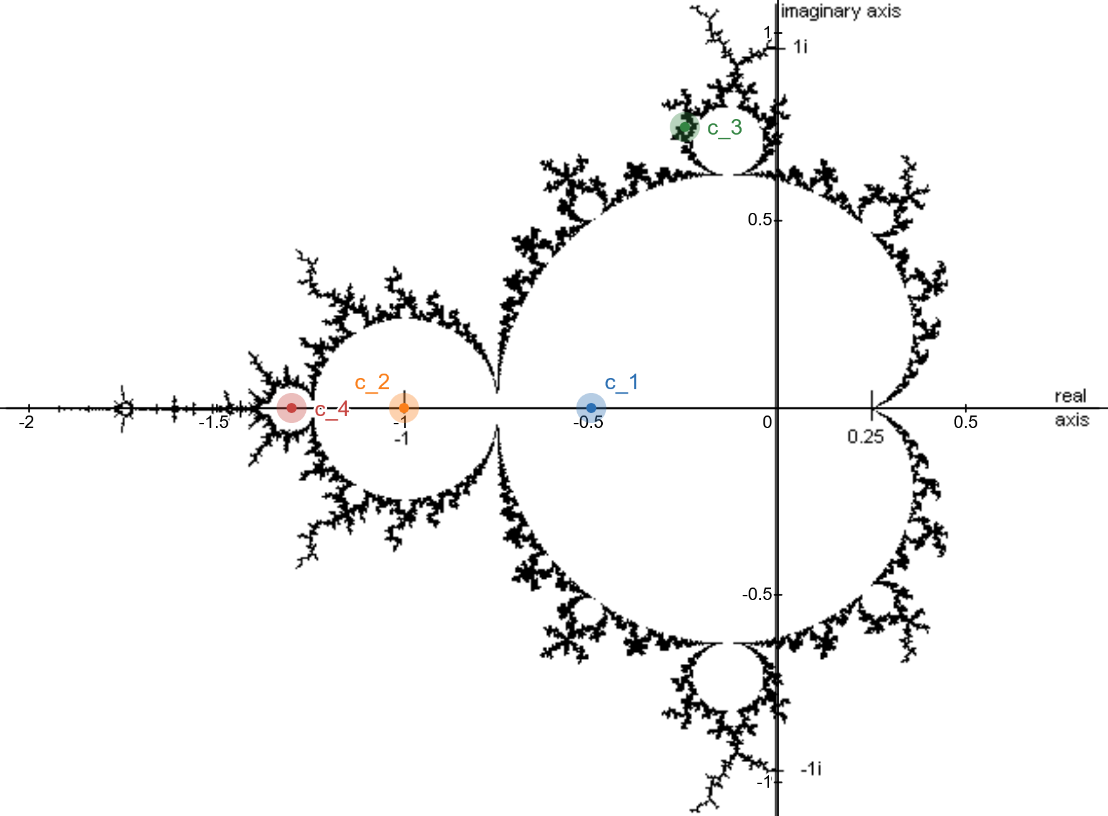
\includegraphics[width=\textwidth]{papers/julia/imgs/mandelbrot_punkte.png}

    \caption{Beispielspunkte in verschiedenen Regionen der Mandelbrot-Menge}
    \label{julia:beispiele_aussehen_mandel}
\end{figure}


\subsection{Verallgemeinerungen}
Die Mandelbrot-Menge lässt sich auf verschiedene Arten verallgemeinern.
In diesem Abschnitt werden einige davon beschrieben.

\subsubsection{Multibrot-Mengen}
Multibrot-Mengen entstehen, wenn man statt einer quadratischen Funktion Polynome eines beliebigen Grades betrachtet
\index{Multibrot-Mengen}%
\begin{equation*}
    f_c(z) = z^d + c.
\end{equation*}
Beispiele davon sind in Abbildung \ref{julia:fig:multibrot_mengen} dargestellt.
Dies kann weiter verallgemeinert werden, indem negative und rationale Zahlen als Exponent $d$ erlaubt werden.
\begin{figure}
    \centering
    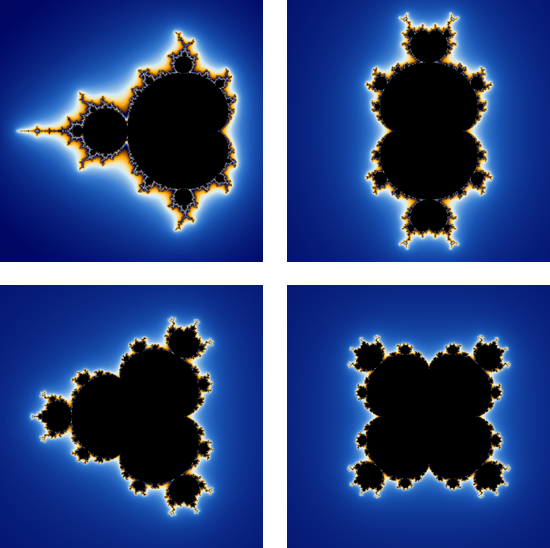
\includegraphics[width=\textwidth]{papers/julia/imgs/multibrot.png}

    \caption{Multibrot-Mengen für Polynome der Grade $2$, $3$, $4$ und $5$}
    \label{julia:fig:multibrot_mengen}
\end{figure}

\subsubsection{Höhere Dimensionen}
Statt den komplexen Zahlen kann auch mit \emph{Quaternionen} gearbeitet werden, diese sind die vierdimensionale Erweiterung der komplexen Zahlen.
\index{Quaternionen}%
Ein Quaternion wird als $q = a + bi + cj + dk$ notiert, mit $i^2 = j^2 = k^2 = ijk = -1$ und $i \ne j \ne k$.

Die vierdimensionale Mandelbrot-Menge kann dann in eine dreidimensionale Struktur projiziert werden, was jedoch relativ uninteressant ist, da es sich lediglich um die Mandelbrot-Menge, rotiert um die reelle Achse handelt \cite{julia:quaternionen}.

\subsubsection{Nicht-analytische Funktionen}
Statt holomorphen Funktionen können auch nicht-holomorphe bzw. nicht-analytische Funktionen verwendet werden.

Ein bekanntes Beispiel ist das Tricorn-Fraktal, dabei wird die Rekursion
\index{Tricorn-Fraktal}%
\begin{equation*}
    z_{n+1} = \overline{z_n}^2 + c
\end{equation*}
verwendet.
Bevor $z_n$ quadriert wird, wird die komplexe Konjugation berechnet.

Ein weiteres Beispiel ist das Burning-Ship-Fraktal, welches durch die Rekursion
\index{Burning-Ship-Fraktal}%
\begin{equation*}
    z_{n+1} = \left(|\text{Re}(z_n)| + i\,|\text{Im}(z_n)|\right)^2 + c
\end{equation*}
entsteht.
Anders als bei der Mandelbrot-Menge werden hier die Beträge des Real- und Imaginärteils berechnet, bevor quadriert wird.

\section{Anwendungen und Zweck}
\label{julia:zweck}
\kopfrechts{Anwendungen und Zweck}%

Die Definitionen für die Julia- und Fatou-Mengen sowie die Mandelbrot-Menge basieren auf interessanten Überlegungen, doch der grundlegende Zweck kann mitunter etwas in den Hintergrund geraten.
Am Anfang des Kapitels wurde mit der Gleichung \eqref{julia:beispielgleichung} und dem Newton-Algorithmus die Überlegung der Funktionen-Iteration motiviert.
Die Iterationsformel \eqref{julia:newton_alg} dieser Gleichung hat zwei Komponenten: die Variable $x_n$ beim Schritt $n$ und den Parameter $a$.
Beide Komponenten lassen sich direkt mit der entwickelten Theorie in Verbindung bringen.

\subsection{Die Variable und die Julia-Mengen}
Für einen fixen Parameterwert $a$ hat die Gleichung \eqref{julia:beispielgleichung} zwei analytische Lösungen: $\!\sqrt{-a}$ und $-\!\sqrt{-a}$.
Weiter ergibt sich aus der Iterationsformel \eqref{julia:newton_alg} die Funktion
\begin{equation*}
    g(x_n) = x_n - \frac{x_n^2 + a}{2x_n} = \frac{x_n^2 - a}{2x_n}.
\end{equation*}
Bei diesen analytischen Lösungen handelt es sich, aus Sicht der Julia-Menge, um Fixpunkte, denn
\begin{equation*}
    g(\!\sqrt{-a}) = \!\sqrt{-a} \qquad \text{und} \qquad g(-\!\sqrt{-a}) = -\!\sqrt{-a}.
\end{equation*}

Möchte man wissen, um welche Art von Fixpunkten es sich handelt, müssen die Werte des Multiplikators \eqref{julia:lambda_multiplicator} für die beiden analytischen Lösungen berechnet werden.
Dazu benötigt man die Ableitung
\begin{equation*}
    \left(g^n\right)^\prime(x_0) = \prod_{k=0}^{n-1} g^\prime\left(g^k(x_0)\right) = g^\prime(x_0) \cdot g^\prime(g(x_0)) \cdot g^\prime(g(g(x_0))) \cdot \ldots
\end{equation*}
und muss diese für die beiden analytischen Lösungen auswerten.
Interessant ist der Faktor $g^\prime(x_0)$, denn sowohl $g^\prime(\!\sqrt{-a})$ als auch $g^\prime(-\!\sqrt{-a})$ sind gleich $0$, wodurch die gesamten Produkte und somit die Multiplikatoren zu $0$ werden.
Gemäss der Definition \ref{julia:lambda_defs} sind daher beide analytischen Lösungen stark anziehende Fixpunkte.

Die komplexe Ebene (oder hier die reellen Zahlen) ist demzufolge in \emph{Einzugsgebiete} unterteilt:
\index{Einzugsgebiet}%
\begin{itemize}
    \item Punkte, für die die Iteration von $g$ zu $\!\sqrt{-a}$ konvergiert
    \item Punkte, für die die Iteration von $g$ zu $-\!\sqrt{-a}$ konvergiert
    \item Punkte, für die die Iteration von $g$ sich anders verhält (z.B. $x = 0$ führt zu Division durch $0$)
\end{itemize}
Die Julia-Menge der Funktion $g$ entspricht genau dem Rand, der diese Einzugsgebiete trennt.
Wählt man einen Punkt auf dem Rand und variiert diesen leicht, fällt man je nach Art der Änderung in unterschiedliche Einzugsgebiete.
Diese Randpunkte verhalten sich also wieder chaotisch.

Möchte man nun die Gleichung \eqref{julia:beispielgleichung} mit der Newton-Iterationsformel \eqref{julia:newton_alg} lösen, benötigt man einen Startwert $x_0$.
Aus Analysis I ist bekannt, dass der Startwert ``genügend nahe'' bei einer Lösung der Gleichung liegen muss.
Berechnet man nun die Julia-Menge der Funktion $g$, findet man so die Einzugsgebiete der Lösungen und kann damit quantifizieren, was ``genügend nahe'' bedeutet.

\subsection{Der Parameter und die Mandelbrot-Menge}
Fixiert man statt dem Parameter, die Variable bei $x_0$, kann so studiert werden, welche Parameterwerte zu welcher Art von Verhalten führen.
Man untersucht nun das Verhalten der Funktion
\begin{equation*}
    g(x_0)_a = \frac{x_0^2 - a}{2x_0}
\end{equation*}
für verschiedene Werte von $a$.
Dies ist analog zur Definition der Mandelbrot-Menge in Abschnitt \ref{julia:sec:mandelbrot} mit dem Unterschied, dass nicht die quadratische Funktion untersucht wird.

Findet man alle Parameterwerte, für die die Rekursion von $g$ beschränkt bleibt, erhält man zwar nicht die klassische Mandelbrot-Menge, aber trotzdem etwas was die gleichen Eigenschaften besitzt.
Hiermit kann also untersucht werden, wie sich verschiedene Parameterwerte $a$ auf das Lösen der Gleichung \eqref{julia:beispielgleichung} mit der Newton-Iterationsformel \eqref{julia:newton_alg} auswirken.

\section{Beziehung zwischen Julia-Mengen und Mandelbrot-Menge}
\label{julia:sec:relation}
\kopfrechts{Beziehung zwischen Julia-Mengen und Mandelbrot-Menge}%

Zwischen der Mandelbrot-Menge sowie den Julia- bzw. Fatou-Mengen bestehen mehrere, teils überraschende Zusammenhänge.
In diesem Abschnitt werden drei solche Zusammenhänge näher betrachtet.

\subsection{Form der Julia-Mengen}
\label{julia:sec:julia_connected}
Anhand der Position in der Mandelbrot-Menge, lässt sich eine Aussage über die Form bzw. das Aussehen der zugehörigen Julia-Menge treffen.
Dafür werden stets Funktionen der Art $f_c(z) = z^2 + c$ betrachtet.

Setzt man zunächst $c = 0$, befindet man sich in der Abbildung \ref{julia:fig:mandelbrot_julia_1} beim weissen Punkt in der Mandelbrot-Menge links.
Rechts daneben ist die Julia-Menge der Funktion $f_c(z) = z^2 + 0$ dargestellt, wobei es sich bekanntlich um den Rand des Einheitskreises handelt.

\begin{figure}
    \centering
    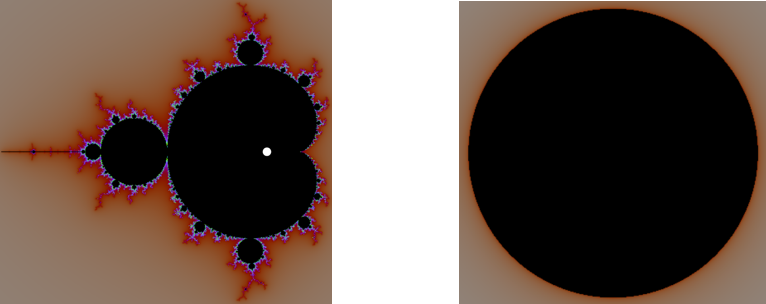
\includegraphics[width=\textwidth]{papers/julia/imgs/mandelbrot_julia_1.png}
    \caption{Mandelbrot-Menge bei $c=0$ und zugehörige Julia-Menge}
    \label{julia:fig:mandelbrot_julia_1}
\end{figure}

Verschiebt man nun $c$ entlang der imaginären Achse, erhält man die Folge von Bildern in den Abbildungen \ref{julia:fig:mandelbrot_julia_2-4} und \ref{julia:fig:mandelbrot_julia_5}.
Links ist jeweils die aktuelle Position des Punktes $c$ dargestellt und rechts die Julia-Menge der Funktion $f_c$ --- parametrisiert mit dem aktuellen $c$.

\begin{figure}
    \centering
    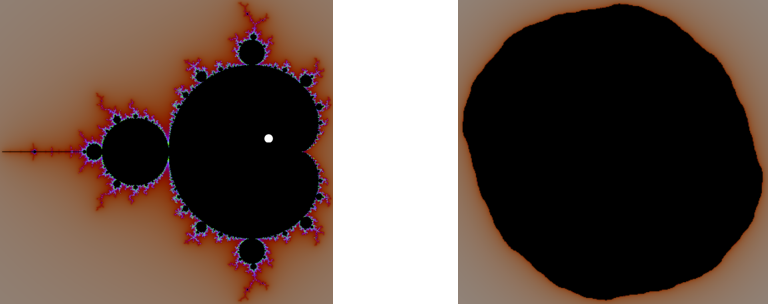
\includegraphics[width=\textwidth]{papers/julia/imgs/mandelbrot_julia_2.png}
    \\[\smallskipamount]
    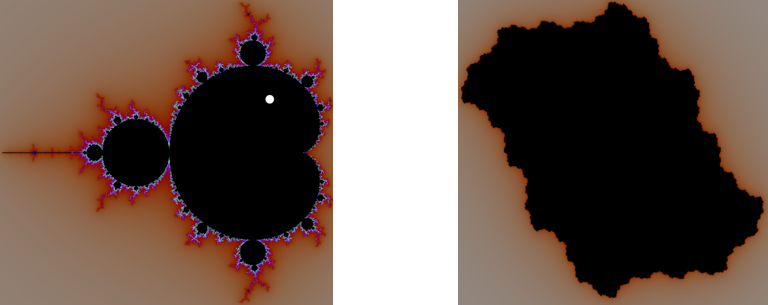
\includegraphics[width=\textwidth]{papers/julia/imgs/mandelbrot_julia_3.png}
    \\[\smallskipamount]
    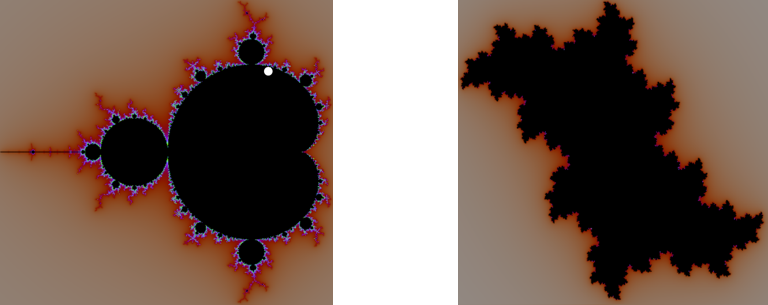
\includegraphics[width=\textwidth]{papers/julia/imgs/mandelbrot_julia_4.png}

    \caption{Mandelbrot-Menge bei $c \in \{\,0.1i,\, 0.4i,\, 0.6i\,\}$ und zugehörige Julia-Mengen}
    \label{julia:fig:mandelbrot_julia_2-4}
\end{figure}

\begin{figure}
    \centering
    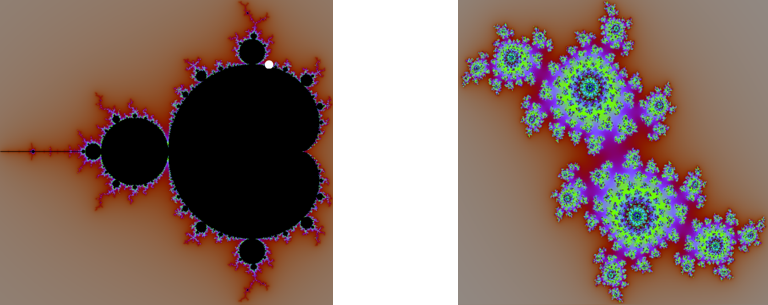
\includegraphics[width=\textwidth]{papers/julia/imgs/mandelbrot_julia_5.png}

    \caption{Mandelbrot-Menge bei $c = 0.65i$, ausserhalb von $M$ und zugehörige Julia-Menge}
    \label{julia:fig:mandelbrot_julia_5}
\end{figure}

Mit änderndem $c$ verformt sich die Julia-Menge zusehends und beim Übergang von $c=0.6i$ zu $c=0.65i$ zerfällt sie.
Grund dafür ist, dass $c=0.6i$ noch in der Mandelbrot-Menge $M$ liegt, während $c=0.65i$ bereits ausserhalb ist.
In den Abbildungen \ref{julia:fig:mandelbrot_julia_2-4} und \ref{julia:fig:mandelbrot_julia_5} ist die Mandelbrot-Menge schwarz dargestellt, alle eingefärbten Punkte gehören nicht mehr dazu.

Es stellt sich heraus, dass die Julia-Menge \emph{zusammenhängend} ist, für alle $c \in M$ und \emph{nicht zusammenhängend} für alle $c \not\in M$.
\index{zusammenhangend@zusammenhängend}%


\subsection{Ähnlichkeit der Mandelbrot- und Julia-Menge}
In der Vergangenheit wurde mehrfach beobachtet, dass Strukturen in der Mandelbrot-Menge ganzen Julia-Mengen ähneln.
Wie sich ergab, tritt für gewisse Arten von Parametern $c$ ein interessantes Phänomen auf.
Dies soll an Funktionen der Art $f_c(z) = z^2 + c$ illustriert werden.

\begin{beispiel}
    Nachfolgend wird der Punkt \[c_1 = 0.3626697754647427\, +\, 0.6450273437137847i\] betrachtet.
    Vergrössert man die Mandelbrot-Menge an diesem Punkt, so ergibt sich die Reihe von Bildern in Abbildung \ref{julia:fig:mandelbrot_zoom}.

    \begin{figure}
        \centering
        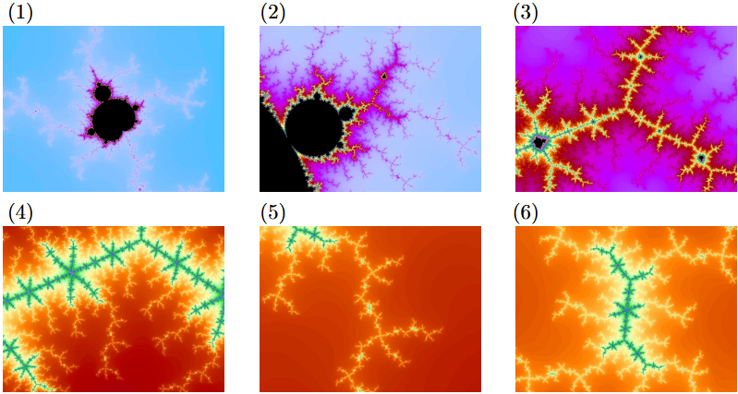
\includegraphics[width=\textwidth]{papers/julia/imgs/mandelbrot_zoom.png}

        \caption{Zoom der Mandelbrot-Menge bei $c_1 = 0.3626697754647427 + 0.6450273437137847i$, vgl. mit Abbildung \ref{julia:fig:julia_zoom} (2)}
        \label{julia:fig:mandelbrot_zoom}
    \end{figure}

    Macht man das gleiche mit der Julia-Menge der Funktion \[f = z^2\, +\, 0.3626697754647427\, +\, 0.6450273437137847i\] ergeben sich die Bilder in Abbildung \ref{julia:fig:julia_zoom}.

    \begin{figure}
        \centering
        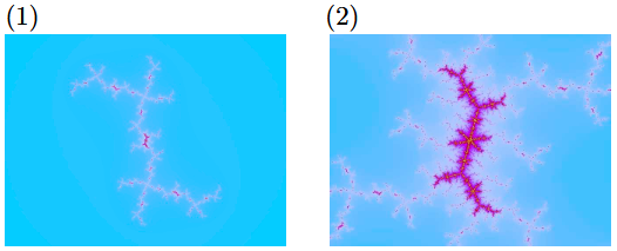
\includegraphics[width=0.65\textwidth]{papers/julia/imgs/julia_zoom.png}

        \caption{Julia-Menge von $f(z) = z^2 + 0.3626697754647427 + 0.6450273437137847i$, vgl. mit Abbildung \ref{julia:fig:mandelbrot_zoom} (6)}
        \label{julia:fig:julia_zoom}
    \end{figure}

    Bis auf das Farbschema und die Ausrichtung sind sind die Bilder (6) der Mandelbrot-Menge und (2) der Julia-Menge fast gleich.
\end{beispiel}

Wie Kawahira und Kisaka in \cite{julia:ähnlichkeit_mandelbrot} gezeigt haben, passiert dies für parabolische Parameter und Misiurewicz-Parameter.
\begin{definition}
    Ein Parameter $c$ wird als \emph{parabolisch} bezeichnet, wenn die Funktion $f_c$ einen periodischen Punkt besitzt, dessen Multiplikator $\lambda$ \eqref{julia:lambda_multiplicator} eine Einheitswurzel (siehe \ref{julia:sec:nicht_fix_periodisch}) ist.
\index{parabolischer Parameter}%
\index{Parameter!parabolisch}%
\end{definition}
\begin{beispiel}
    Ein Beispiel ist der Parameter $c = \frac{1}{4}$.
    Die Funktion $f(z) = z^2 + \frac{1}{4}$ besitzt einen Fixpunkt bei $z_0 = \frac{1}{2}$, denn $f(z_0) = \left(\frac{1}{2}\right)^2 + \frac{1}{4} = z_0$.
    Weiter ist $\lambda = \left(f\right)^\prime(z_0) = 2 z_0 = 1$, wobei es sich um eine Einheitswurzel handelt.
\end{beispiel}

\begin{definition}
    Ein Parameter $c$ heisst \emph{Misiurewicz-Parameter}, wenn der Startwert $z_0 = 0$ präperiodisch, aber nicht periodisch ist.
\index{Misiurewicz-Parameter}%
\index{Parameter!Misiurewicz-}%
\end{definition}
Ein präperiodischer Startwert wird nach endlich vielen Iterationen periodisch, ist aber selbst nicht periodisch.
Dies ist dargestellt in Abbildung \ref{julia:fig:preperiodic}.

\begin{figure}
    \centering
    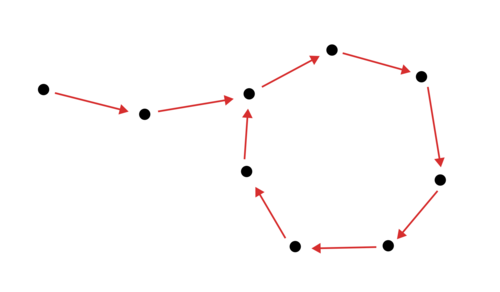
\includegraphics[width=0.6\textwidth]{papers/julia/imgs/preperiodic.png}

    \caption{Ein Zyklus ausgehend von einem präperiodischen Startwert}
    \label{julia:fig:preperiodic}
\end{figure}

\begin{beispiel}
    Beim Parameter $c = -2$ handelt es sich um einen Misiurewicz-Parameter, iteriert man die Funktion $f_c$ ausgehend von $z_0 = 0$, ergibt sich die Folge
    \begin{equation*}
        0 \mapsto -2 \mapsto 2 \mapsto 2 \mapsto 2 \mapsto \ldots\, .
    \end{equation*}
    Diese Folge wird ab der dritten Iteration periodisch.
\end{beispiel}


\subsection{Mosaik der Mandelbrot-Menge}
Werden Julia-Mengen auf eine bestimmte Art angeordnet, ergibt sich ein Mosaik der Mandelbrot-Menge.
Dazu legt man ein Gitter über die Mandelbrot-Menge und wählt einen Gitterpunkt aus, illustriert in der Abbildung \ref{julia:fig:mosaik1}.

\begin{figure}
    \centering
    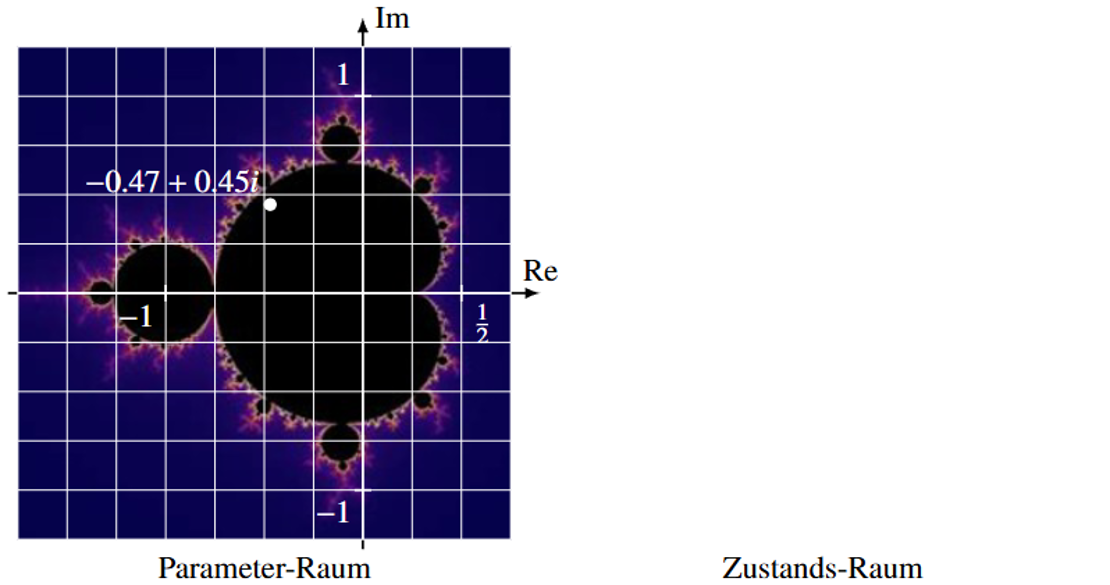
\includegraphics[width=0.95\textwidth]{papers/julia/imgs/mosaik1.png}

    \caption{Gitterpunkt $-0.47 + 0.45i$ in der Mandelbrot-Menge}
    \label{julia:fig:mosaik1}
\end{figure}

Mit dem gewählten Parameter $c = -0.47 + 0.45i$ berechnet man nun die Julia-Menge der Funktion $f(z) = z^2 - 0.47 + 0.45i$.
Die Julia-Menge wird nun in das Gitter platziert und zwar an den Ort des Parameters $c$.
Anschliessend wird sie verkleinert, dies ist in Abbildung \ref{julia:fig:mosaik2-4} dargestellt.
Nun wird dieser Vorgang für sämtliche Gitterpunkte wiederholt, wodurch Abbildung \ref{julia:fig:mosaik5} entsteht.

\begin{figure}
    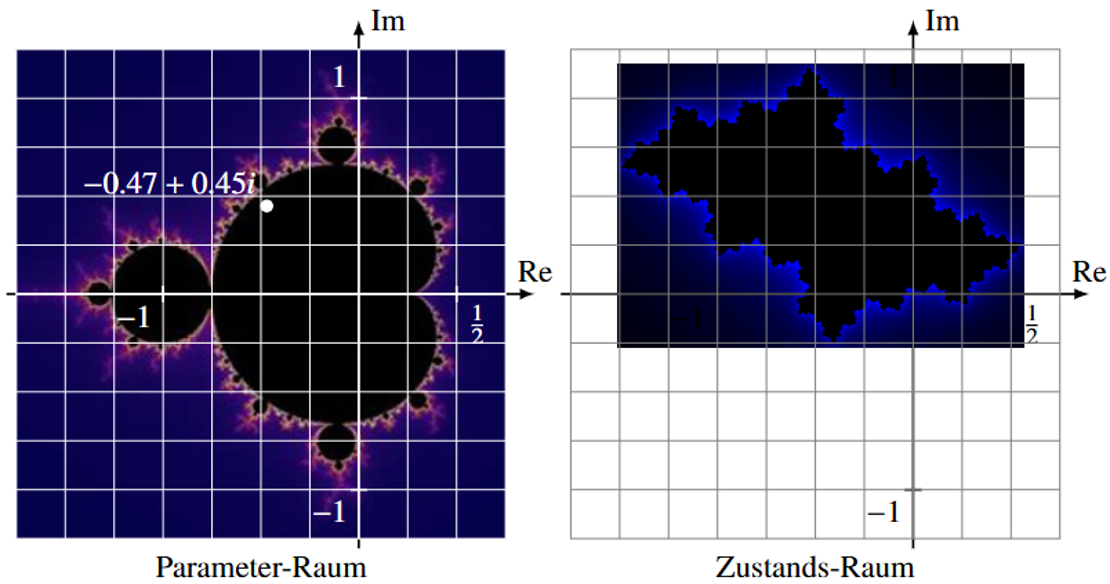
\includegraphics[width=0.95\textwidth]{papers/julia/imgs/mosaik2.png}
    \\[\smallskipamount]
    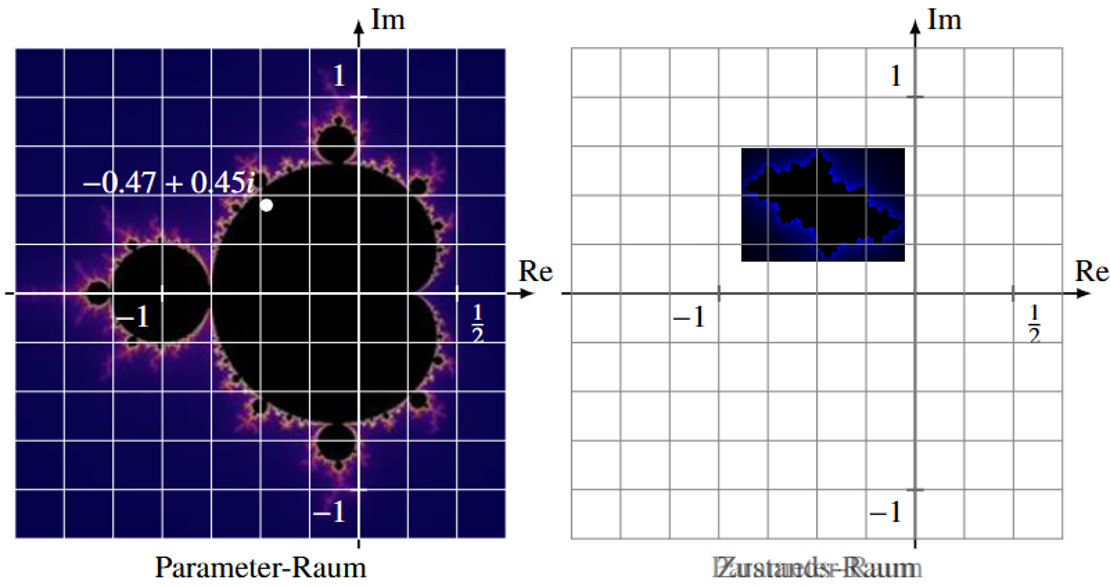
\includegraphics[width=0.95\textwidth]{papers/julia/imgs/mosaik3.png}
    \\[\smallskipamount]
    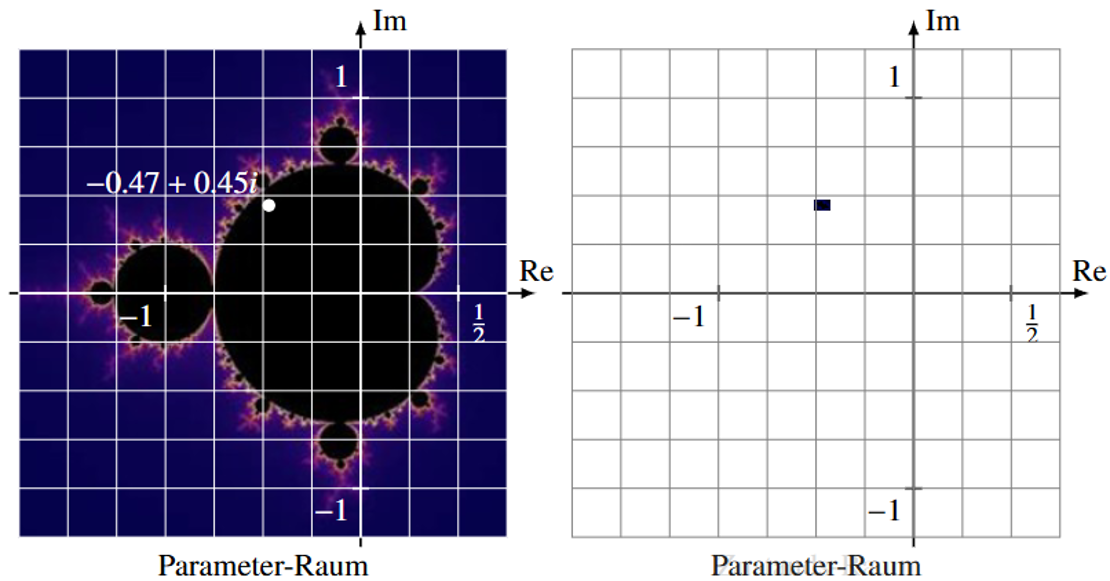
\includegraphics[width=0.95\textwidth]{papers/julia/imgs/mosaik4.png}

    \caption{Kleiner werdende Julia-Menge der Funktion $f(z) = z^2 - 0.47 + 0.45i$ am Punkt $-0.47 + 0.45i$}
    \label{julia:fig:mosaik2-4}
\end{figure}

\begin{figure}
    \centering
    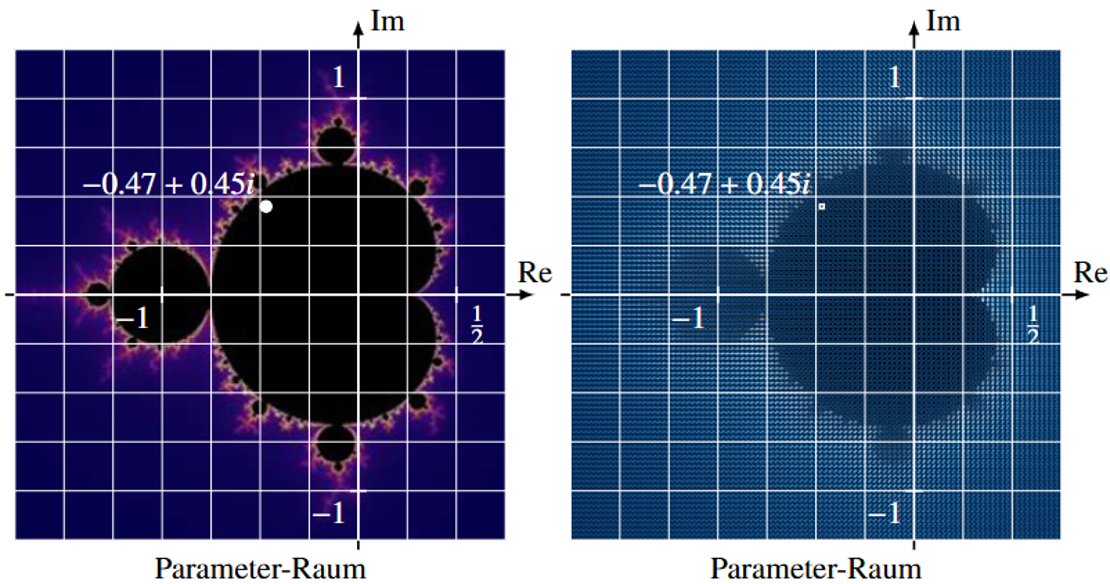
\includegraphics[width=0.95\textwidth]{papers/julia/imgs/mosaik5.png}

    \caption{Mosaik der Mandelbrot-Menge bestehend aus $100$ mal $100$ Julia-Mengen}
    \label{julia:fig:mosaik5}
\end{figure}

Aus dem Zustandsraum, in dem die Julia-Mengen existieren, wurde der Parameterraum nachgestellt, in dem die Mandelbrot-Menge existiert.
Der Grund für dieses Resultat ist, dass die Mandelbrot-Menge eine Art ``Katalog'' sämtlicher Julia-Mengen bildet.

\section{Visualisierung der Mengen}
\label{julia:sec:visualisierung}
\kopfrechts{Visualisierung der Mengen}%
In den vorherigen Abschnitten wurden Bilder von der Mandelbrot-Menge sowie der Julia- und Fatou-Mengen gezeigt.
Nachfolgend wird beschrieben wie diese Mengen visualisiert werden.
Bei diesen Visualisierungen handelt es sich um \emph{Fraktale}, was bedeutet dass, unabhängig vom Vergrösserungsfaktor, stets neue Details und Strukturen erscheinen.
\index{Fraktal}%
Diese Strukturen sind häufig selbstähnlich, heisst sie sind eingebettet in grössere Strukturen, die ähnlich aussehen.
\index{selbstähnlich}%

\subsection{Visualisierung der Julia- und Fatou-Mengen}

\begin{aufgabe}
    Visualisierung einer Julia- und Fatou-Menge
    \begin{enumerate}
        \item Funktion $f(z)$ wählen
        \item Die reelle und imaginäre Achse der $z$-Ebene plotten
        \item $f^n(z_i)$ für jeden Punkt $z_i$ dieses Koordinatensystems berechnen
        \item Punkte $z_i$ einfärben, je nachdem wie schnell und ob sie divergieren
    \end{enumerate}
\end{aufgabe}
Zu beachten ist, dass $n$ in der Theorie gegen unendlich geht, in der Praxis ist dies natürlich nicht möglich, je nach Rechenleistung muss ein genügend grosser Wert für $n$ gewählt werden.

Je nach gewählter Funktion und Farbschema können so sehr eindrückliche Bilder erstellt werden, wie zum Beispiel in Abbildung \ref{julia:fig:bsp_julia}.
Interessant wird es besonders dann, wenn die Julia-Menge nicht zusammenhängend ist (siehe Abschnitt \ref{julia:sec:julia_connected}).
In diesem Fall besteht die Julia-Menge häufig nur aus einzelnen Punkten, während die übrigen Punkte zur Fatou-Menge gehören.

\begin{figure}
    \centering
    
\includegraphics[width=0.95\textwidth]{papers/julia/imgs/julia3.jpg}

    \caption{Beispiel einer Julia-Menge der Funktion $f(z) = z^2 + c$ für einen Parameter $c$ nahe des Randes der Mandelbrot-Menge}
    \label{julia:fig:bsp_julia}
\end{figure}

\subsection{Visualisierung der Mandelbrot-Menge}
\label{julia:sec:visualisierung_mandel}

\begin{aufgabe}
    Visualisierung der Mandelbrot-Menge
    \begin{enumerate}
        \item Beginne mit $f_c(z) = z^2 + c$
        \item Die reelle und imaginäre Achse der $c$-Ebene plotten
        \item $f^n_{c_i}(0)$ für jeden Punkt $c_i$ dieses Koordinatensystems berechnen
        \item Punkte $c_i$ einfärben, je nachdem wie schnell und ob sie divergieren
    \end{enumerate}
\end{aufgabe}
Der Ablauf ist im wesentlichen gleich wie bei den Julia- und Fatou-Mengen, der grosse Unterschied liegt darin, dass hier der Parameterraum bzw. die $c$-Ebene abgebildet wird.
Auch hier gilt in der Theorie $n \to \infty$, es muss wieder ein genügend grosser Wert für $n$ gewählt werden.

Je nach Farbschema führt auch dies zu sehr eindrücklichen Bildern, wie zum Beispiel Abbildung \ref{julia:fig:bsp_mandelbrot}.

\begin{figure}
    \centering
    
\includegraphics[width=0.95\textwidth]{papers/julia/imgs/mandelbrot1.jpg}

    \caption{Herausgezoomtes und leicht rotiertes Beispiel der Mandelbrot-Menge}
    \label{julia:fig:bsp_mandelbrot}
\end{figure}



\printbibliography[heading=subbibliography]
\end{refsection}
